\section{Observation and Calculations}

Figs. \ref{znte}a, \ref{cds}a and \ref{zno}a show the absorbance vs. wavelength plots obtained from the spectrometer for three materials -- ZnTe, CdS and ZnO. All the materials used in this experiment are direct band gap materials.

\begin{figure}
    % \ContinuedFloat
    % \bigskip
    \begin{subfigure}{\linewidth}
    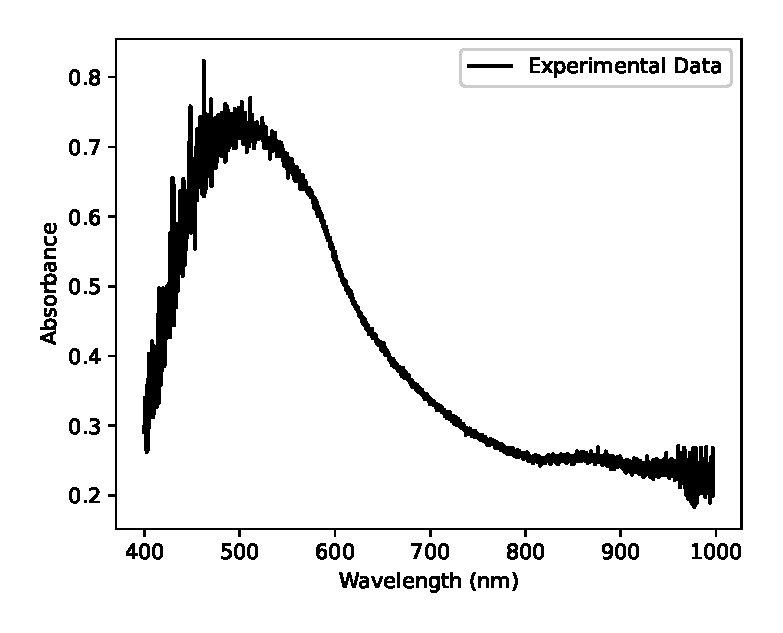
\includegraphics[width=1\textwidth]{images/znteA.eps}
    \caption{Absorbance vs. Wavelength}
    \end{subfigure}
    
    % \bigskip
    \begin{subfigure}{\linewidth}
    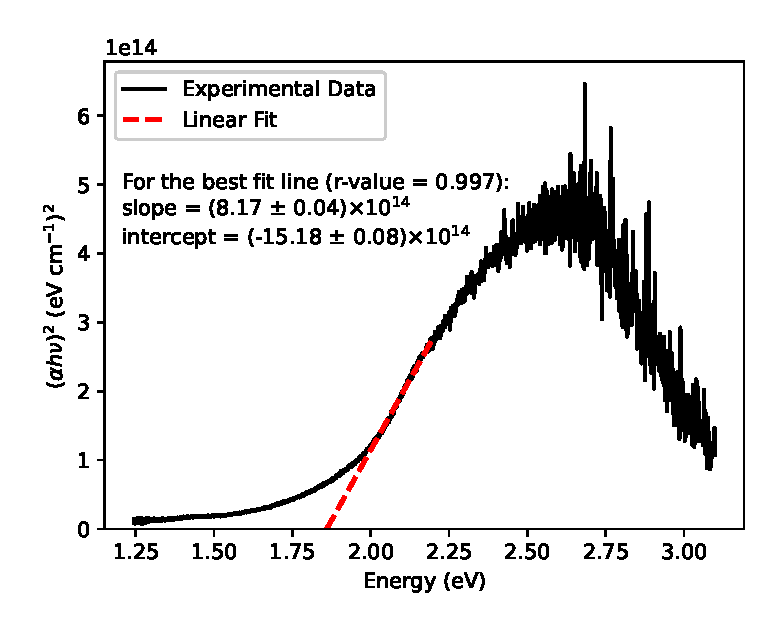
\includegraphics[width=1\textwidth]{images/znte.eps}
    \caption{$(\alpha h \nu)^2$ vs. Energy}
    \end{subfigure}
    \caption{Absorbance plots for ZnTe}
    \label{znte}
\end{figure}

\begin{figure}
    % \ContinuedFloat
    % \bigskip
    \begin{subfigure}{\linewidth}
    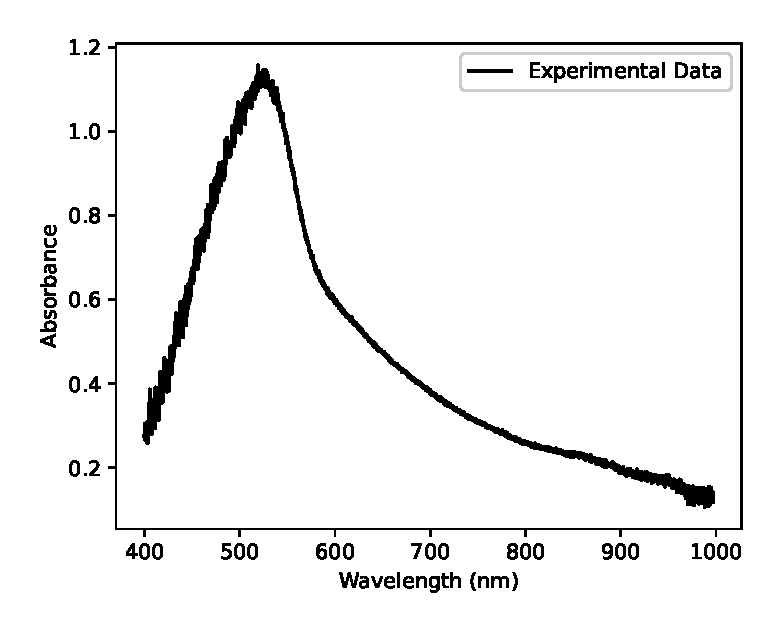
\includegraphics[width=1\textwidth]{images/cdsA.eps}
    \caption{Absorbance vs. Wavelength}
    \end{subfigure}
    
    % \bigskip
    \begin{subfigure}{\linewidth}
    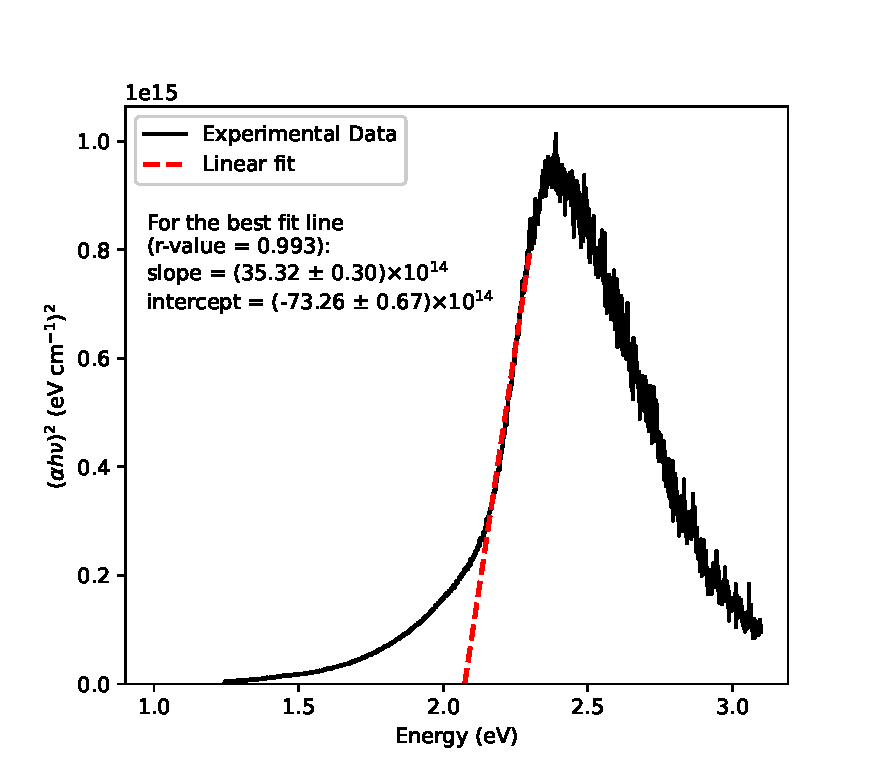
\includegraphics[width=1\textwidth]{images/cds.eps}
    \caption{$(\alpha h \nu)^2$ vs. Energy}
    \end{subfigure}
    \caption{Absorbance plots for ZnTe}
    \label{cds}
\end{figure}

\begin{figure}
    % \ContinuedFloat
    % \bigskip
    \begin{subfigure}{\linewidth}
    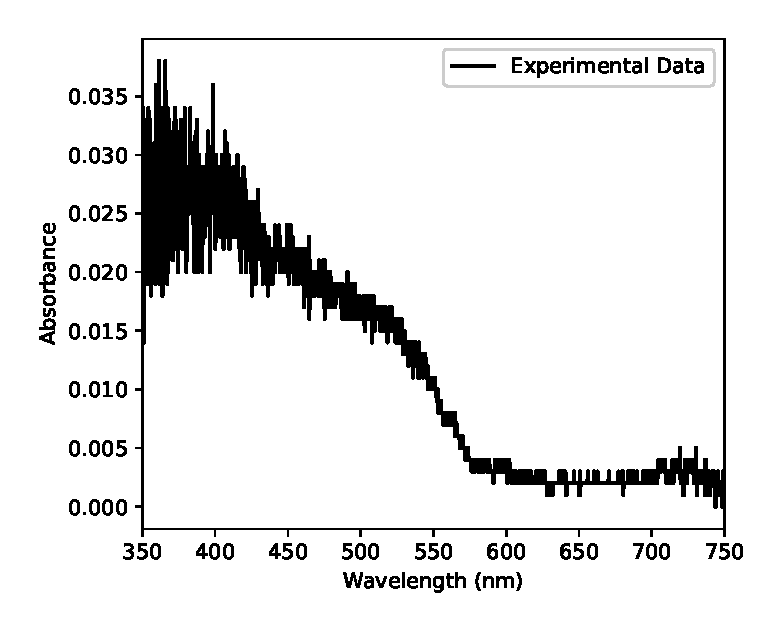
\includegraphics[width=1\textwidth]{images/znoA.eps}
    \caption{Absorbance vs. Wavelength}
    \end{subfigure}
    
    % \bigskip
    \begin{subfigure}{\linewidth}
    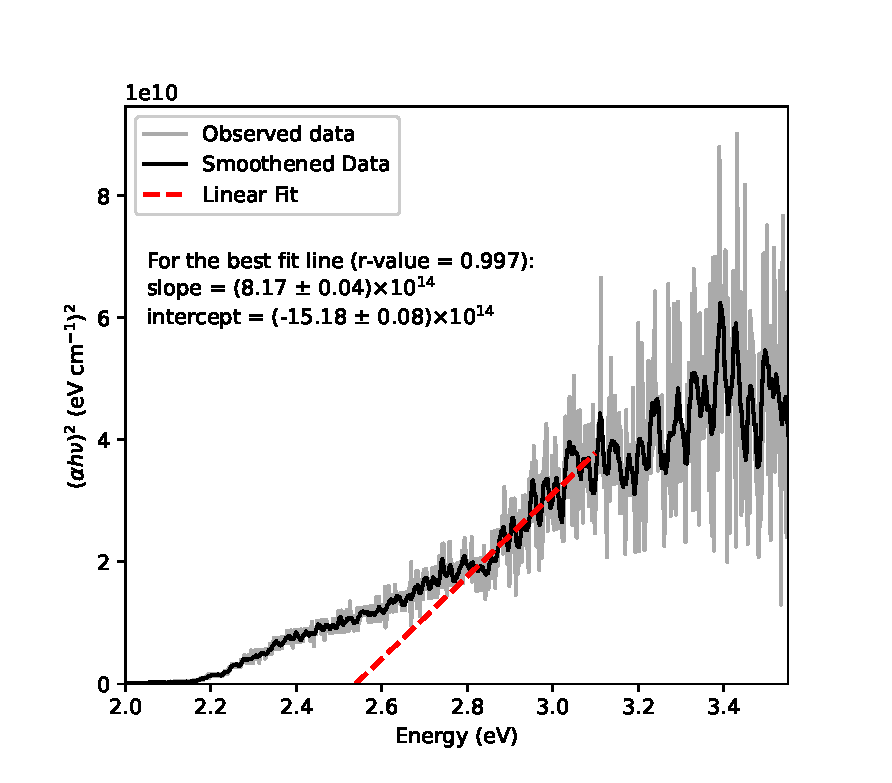
\includegraphics[width=1\textwidth]{images/zno.eps}
    \caption{$(\alpha h \nu)^2$ vs. Energy}
    \label{znob}
    \end{subfigure}
    \caption{Absorbance plots for ZnTe}
    \label{zno}
\end{figure}

Using the obtained values of $A$, we have calculated $\alpha$ using Eq. \ref{1}. Figs. \ref{znte}b, \ref{cds}b and \ref{znob} show the $(\alpha h \nu)^{2}$ vs. $h\nu$ plots for ZnTe, CdS and ZnO respectively.  By fitting a straight line over the linear region we have obtained the slope and intercept parameters. We have used the Savitzky–Golay filter for ZnO to smoothen the plot as the experimental data had a very high signal to noise ratio. 

Eq. \ref{directeq} can be rewritten as

\begin{align}
    (\alpha h \nu)^{2} = Ah\nu - AE_g
\end{align}

Here, $AE_g$ is the y-intercept and hence $AE_g/A=E_g$ will be the $x$-intercept of the linear region.

The $x$-intercept can be calculated by taking the ratio of the intercept to the slope. The corresponding $x$-intercepts, which represent the band-gap energies are:

\begin{itemize}
    \item For ZnTe: 1.859 eV
    \item For CdS: 2.074 eV
    \item For ZnO: 2.539 eV
\end{itemize}

\section{Error Analysis}

The error in the estimation of $E_g$ can be calulated from the uncertainities in the slope and intercept of the linear region.

\begin{align}
\frac{\Delta E_g}{E_g} = \sqrt{\left(\frac{\Delta \text{slope}}{\text{slope}}\right)^2 + \left(\frac{\Delta \text{intercept}}{\text{intercept}}\right)^2}
\end{align}

Plugging in the values for all three plots, the corresponding $\Delta E_g$'s are:
\begin{itemize}
    \item For ZnTe: 0.026 eV
    \item For CdS: 0.013 eV
    \item For ZnO: 0.359 eV
\end{itemize}